% --- Foundation models: definition, impact, types, and adaptation ---
% --- What are Foundation Models? ---
\begin{frame}{What are Foundation Models?}
  \begin{itemize}
    \item \textbf{Foundation models} are large, general AI models pretrained on massive, diverse datasets.
    \item They provide a universal base that can be adapted (via fine-tuning or prompting) across many domains and tasks.
    \item The key shift: build powerful, flexible models for reuse, rather than training a new model for each task from scratch.
  \end{itemize}
  \centering
  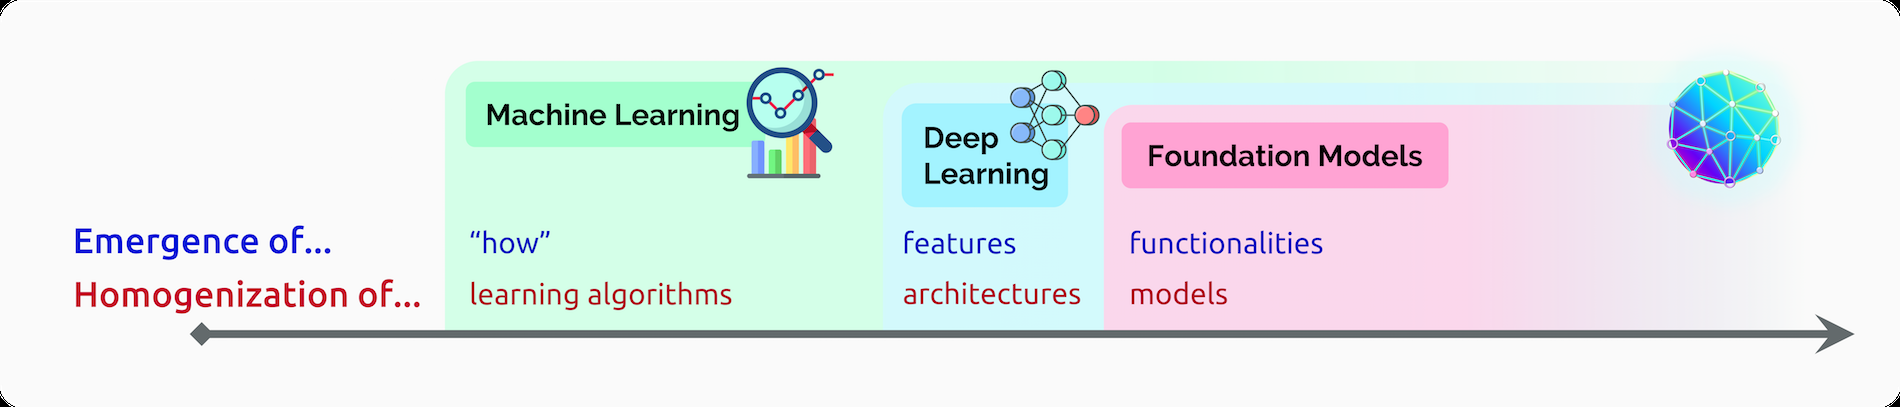
\includegraphics[width=0.98\textwidth]{assets/New-Lecture_Foundation_models/crfm2108_fig1_emergence_homogenization.png}\\[0.1em]
  {\scriptsize Emergence and homogenization from ML $\rightarrow$ deep learning $\rightarrow$ foundation models (Bommasani et al., arXiv:2108.07258).}
\end{frame}

% --- Why Foundation Models? Their Impact ---
\begin{frame}{Why Do Foundation Models Matter?}
  \begin{itemize}
    \item \textbf{Accelerate innovation:} Dramatically reduce time and resources needed to create high-performing AI applications.
    \item \textbf{Expand accessibility:} Lower the expertise required for deploying AI, empowering domain experts (not just AI researchers).
    \item \textbf{Enable new capabilities:} Support advanced “few-shot” and “zero-shot” learning, allowing for rapid adaptation to new tasks.
    \item \textbf{Transform industries:} Fuel advances in medicine, science, robotics, business, and beyond.
    \item \textbf{Introduce new challenges:} Require careful management of data/computational resources, fairness, safety, and responsible use.
  \end{itemize}
\end{frame}

\begin{frame}{How Do Foundation Models Work?}
  \centering
  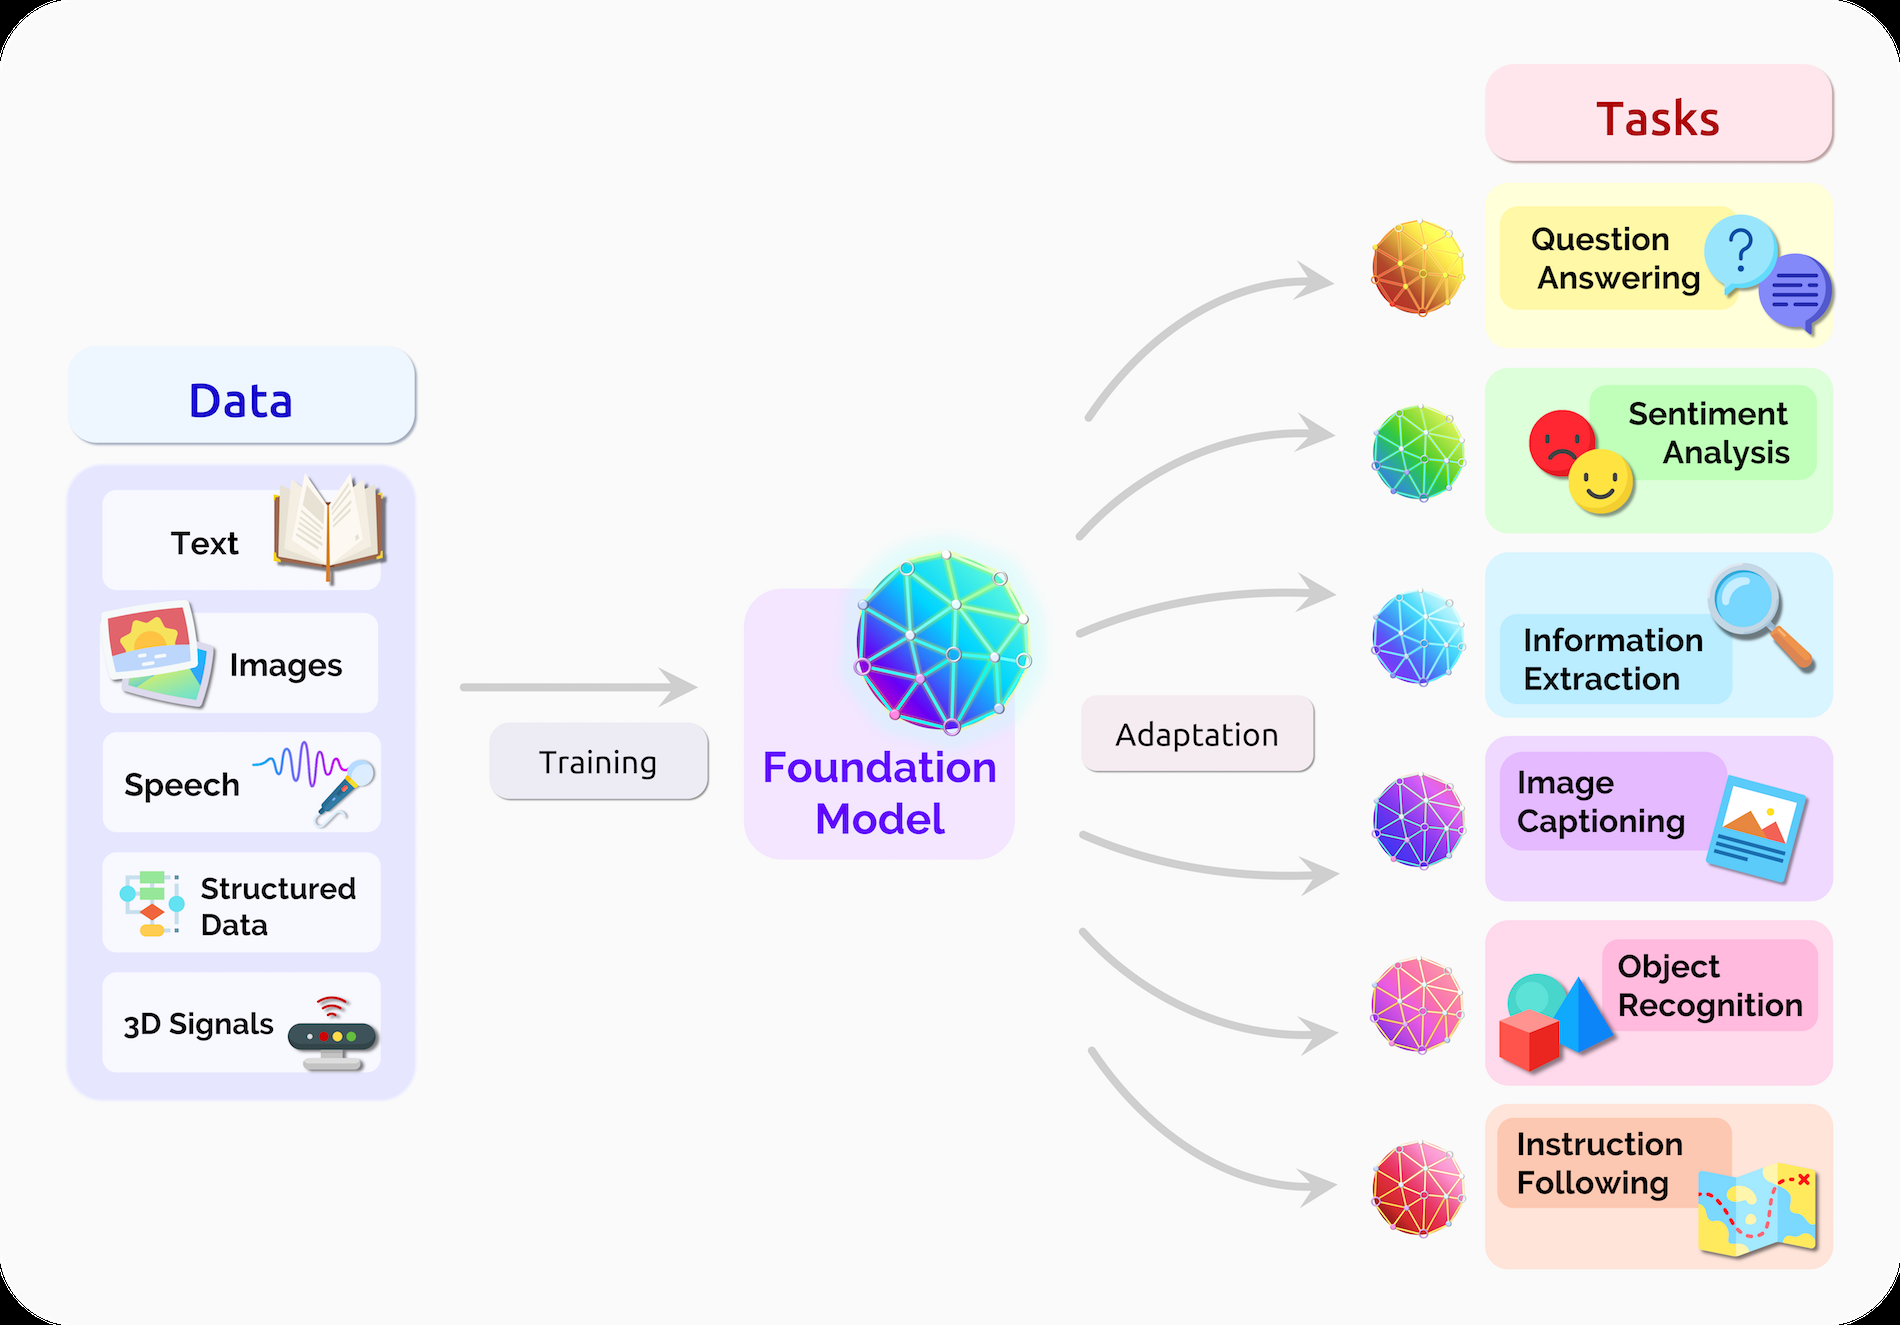
\includegraphics[width=0.92\textwidth]{assets/New-Lecture_Foundation_models/crfm2108_fig2_modalities_to_tasks.png}\\[0.1em]
  {\scriptsize Diverse modalities feed training; one foundation model supports many downstream tasks via adaptation (Bommasani et al., arXiv:2108.07258).}
\end{frame}

% --- Types of Foundation Models ---
\begin{frame}{Types of Foundation Models}
  \begin{itemize}
    \item \textbf{Language models:} Trained on text data, these models can generate, summarize, and understand language.\\
      {\footnotesize Examples: BERT, GPT}
    \item \textbf{Vision models:} Trained on images/videos, they can recognize objects, segment scenes, and more.\\
      {\footnotesize Examples: CLIP, SAM}
    \item \textbf{Multi-modal models:} Learn to connect information across text, images, audio, or video.\\
      {\footnotesize Examples: CLIP (text-image), Flamingo, Gemini}
    \item \textbf{Other domains:} Foundation models exist for structured (tabular) data, medical data, code, and scientific domains.
  \end{itemize}
\end{frame}

% --- How Do Foundation Models Work? ---
\begin{frame}{How Do Foundation Models Work?}
  \begin{itemize}\footnotesize
    \item \textbf{Pretraining at scale:} Train on enormous datasets (text, images, etc.) using self-supervision; learn generalized representations.
    \item \textbf{Adaptation:} Foundation models can be quickly adapted to new tasks using:
      \begin{itemize}
        \item Fine-tuning on small amounts of labeled data
        \item Prompting (providing instructions or context)
        \item In-context learning (few-shot or zero-shot)
      \end{itemize}
    \item \textbf{Transfer learning:} Reuse knowledge across tasks and domains, reducing the need for bespoke model training.
    \item \textbf{Unified architectures:} Many foundation models use architectures like transformers, enabling processing across modalities.
  \end{itemize}
\end{frame}

% --- Examples of Foundation Models ---
\begin{frame}{Examples of Foundation Models}
  \begin{itemize}
    \item \textbf{BERT:} Foundation for language understanding and search.
    \item \textbf{GPT (Generative Pretrained Transformer):} Powers chatbots, writing assistants, and more.
    \item \textbf{CLIP:} Bridges vision and language—for example, “find images matching this caption.”
    \item \textbf{SAM (Segment Anything Model):} Segments objects in any image with a single forward pass.
    \item \textbf{Gemini (Google):} Multi-modal model that integrates language, vision, and more.
    \item \textbf{PaLM, LaMDA, Imagen:} Other prominent foundation models from industry leaders.
  \end{itemize}
\end{frame}
